% Options for packages loaded elsewhere
\PassOptionsToPackage{unicode}{hyperref}
\PassOptionsToPackage{hyphens}{url}
\PassOptionsToPackage{dvipsnames,svgnames,x11names}{xcolor}
%
\documentclass[
]{article}

\usepackage{amsmath,amssymb}
\usepackage{lmodern}
\usepackage{iftex}
\ifPDFTeX
  \usepackage[T1]{fontenc}
  \usepackage[utf8]{inputenc}
  \usepackage{textcomp} % provide euro and other symbols
\else % if luatex or xetex
  \usepackage{unicode-math}
  \defaultfontfeatures{Scale=MatchLowercase}
  \defaultfontfeatures[\rmfamily]{Ligatures=TeX,Scale=1}
\fi
% Use upquote if available, for straight quotes in verbatim environments
\IfFileExists{upquote.sty}{\usepackage{upquote}}{}
\IfFileExists{microtype.sty}{% use microtype if available
  \usepackage[]{microtype}
  \UseMicrotypeSet[protrusion]{basicmath} % disable protrusion for tt fonts
}{}
\makeatletter
\@ifundefined{KOMAClassName}{% if non-KOMA class
  \IfFileExists{parskip.sty}{%
    \usepackage{parskip}
  }{% else
    \setlength{\parindent}{0pt}
    \setlength{\parskip}{6pt plus 2pt minus 1pt}}
}{% if KOMA class
  \KOMAoptions{parskip=half}}
\makeatother
\usepackage{xcolor}
\setlength{\emergencystretch}{3em} % prevent overfull lines
\setcounter{secnumdepth}{-\maxdimen} % remove section numbering
% Make \paragraph and \subparagraph free-standing
\ifx\paragraph\undefined\else
  \let\oldparagraph\paragraph
  \renewcommand{\paragraph}[1]{\oldparagraph{#1}\mbox{}}
\fi
\ifx\subparagraph\undefined\else
  \let\oldsubparagraph\subparagraph
  \renewcommand{\subparagraph}[1]{\oldsubparagraph{#1}\mbox{}}
\fi


\providecommand{\tightlist}{%
  \setlength{\itemsep}{0pt}\setlength{\parskip}{0pt}}\usepackage{longtable,booktabs,array}
\usepackage{calc} % for calculating minipage widths
% Correct order of tables after \paragraph or \subparagraph
\usepackage{etoolbox}
\makeatletter
\patchcmd\longtable{\par}{\if@noskipsec\mbox{}\fi\par}{}{}
\makeatother
% Allow footnotes in longtable head/foot
\IfFileExists{footnotehyper.sty}{\usepackage{footnotehyper}}{\usepackage{footnote}}
\makesavenoteenv{longtable}
\usepackage{graphicx}
\makeatletter
\def\maxwidth{\ifdim\Gin@nat@width>\linewidth\linewidth\else\Gin@nat@width\fi}
\def\maxheight{\ifdim\Gin@nat@height>\textheight\textheight\else\Gin@nat@height\fi}
\makeatother
% Scale images if necessary, so that they will not overflow the page
% margins by default, and it is still possible to overwrite the defaults
% using explicit options in \includegraphics[width, height, ...]{}
\setkeys{Gin}{width=\maxwidth,height=\maxheight,keepaspectratio}
% Set default figure placement to htbp
\makeatletter
\def\fps@figure{htbp}
\makeatother
\newlength{\cslhangindent}
\setlength{\cslhangindent}{1.5em}
\newlength{\csllabelwidth}
\setlength{\csllabelwidth}{3em}
\newlength{\cslentryspacingunit} % times entry-spacing
\setlength{\cslentryspacingunit}{\parskip}
\newenvironment{CSLReferences}[2] % #1 hanging-ident, #2 entry spacing
 {% don't indent paragraphs
  \setlength{\parindent}{0pt}
  % turn on hanging indent if param 1 is 1
  \ifodd #1
  \let\oldpar\par
  \def\par{\hangindent=\cslhangindent\oldpar}
  \fi
  % set entry spacing
  \setlength{\parskip}{#2\cslentryspacingunit}
 }%
 {}
\usepackage{calc}
\newcommand{\CSLBlock}[1]{#1\hfill\break}
\newcommand{\CSLLeftMargin}[1]{\parbox[t]{\csllabelwidth}{#1}}
\newcommand{\CSLRightInline}[1]{\parbox[t]{\linewidth - \csllabelwidth}{#1}\break}
\newcommand{\CSLIndent}[1]{\hspace{\cslhangindent}#1}

\makeatletter
\makeatother
\makeatletter
\makeatother
\makeatletter
\@ifpackageloaded{caption}{}{\usepackage{caption}}
\AtBeginDocument{%
\ifdefined\contentsname
  \renewcommand*\contentsname{Table of contents}
\else
  \newcommand\contentsname{Table of contents}
\fi
\ifdefined\listfigurename
  \renewcommand*\listfigurename{List of Figures}
\else
  \newcommand\listfigurename{List of Figures}
\fi
\ifdefined\listtablename
  \renewcommand*\listtablename{List of Tables}
\else
  \newcommand\listtablename{List of Tables}
\fi
\ifdefined\figurename
  \renewcommand*\figurename{Figure}
\else
  \newcommand\figurename{Figure}
\fi
\ifdefined\tablename
  \renewcommand*\tablename{Table}
\else
  \newcommand\tablename{Table}
\fi
}
\@ifpackageloaded{float}{}{\usepackage{float}}
\floatstyle{ruled}
\@ifundefined{c@chapter}{\newfloat{codelisting}{h}{lop}}{\newfloat{codelisting}{h}{lop}[chapter]}
\floatname{codelisting}{Listing}
\newcommand*\listoflistings{\listof{codelisting}{List of Listings}}
\makeatother
\makeatletter
\@ifpackageloaded{caption}{}{\usepackage{caption}}
\@ifpackageloaded{subcaption}{}{\usepackage{subcaption}}
\makeatother
\makeatletter
\@ifpackageloaded{tcolorbox}{}{\usepackage[many]{tcolorbox}}
\makeatother
\makeatletter
\@ifundefined{shadecolor}{\definecolor{shadecolor}{rgb}{.97, .97, .97}}
\makeatother
\makeatletter
\makeatother
\ifLuaTeX
  \usepackage{selnolig}  % disable illegal ligatures
\fi
\IfFileExists{bookmark.sty}{\usepackage{bookmark}}{\usepackage{hyperref}}
\IfFileExists{xurl.sty}{\usepackage{xurl}}{} % add URL line breaks if available
\urlstyle{same} % disable monospaced font for URLs
\hypersetup{
  pdftitle={TBD},
  colorlinks=true,
  linkcolor={blue},
  filecolor={Maroon},
  citecolor={Blue},
  urlcolor={Blue},
  pdfcreator={LaTeX via pandoc}}

\title{TBD}
\author{true}
\date{}

\begin{document}
\maketitle
\begin{abstract}
This is the abstract for the paper.
\end{abstract}
\ifdefined\Shaded\renewenvironment{Shaded}{\begin{tcolorbox}[boxrule=0pt, sharp corners, interior hidden, borderline west={3pt}{0pt}{shadecolor}, enhanced, breakable, frame hidden]}{\end{tcolorbox}}\fi

\hypertarget{introduction}{%
\section{Introduction}\label{introduction}}

Dental calculus is quickly becoming the go-to substance for exploring
health and diet in past populations. Studies using archaeological dental
calculus span a wide range of topics in different regions and time
periods. These include characterisation of the oral microbiome and its
evolution in past populations (Velsko et al. 2019; Adler et al. 2013;
Warinner et al. 2014; Kazarina et al. 2021; Fellows Yates et al. 2021),
extraction of microbotanical remains (Henry and Piperno 2008; Hardy et
al. 2009; Mickleburgh and Pagán-Jiménez 2012; \textbf{maHumanDiet2022?})
and other residues to infer dietary patterns and nicotine-use (Buckley
et al. 2014; Hendy et al. 2018; Eerkens et al. 2018).

Dental calculus is formed by the mineralisation of dental plaque. Dental
plaque is an oral biofilm and is part of the normal state of the oral
cavity; however, if left unchecked, plaque can lead to infections such
as dental caries and periodontitis (Marsh 2006). Shortly after teeth are
cleaned (whether mechanically or otherwise), a salivary pellicle adsorbs
to the surface of the tooth, in most cases enamel, forming the acquired
dental pellicle. The pellicle is comprised mainly of proteins and, in
addition to protecting the tooth against mechanical and chemical decay,
provides a viable surface for bacterial attachment
(\textbf{yaoIdentificationProtein2003?}). Shortly after adsorbing to the
enamel, early-coloniser species, such as those within genus
\emph{Streptococcus} and \emph{Actinomyces}, adhere to the pellicle
through reversible long-range physicochemical forces and irreversible
short range cell-host interactions (Marsh 2006). Once the surface has
been populated by the specialists in surface-attachment, other species
of bacteria can attach to their surface through cell-cell interactions,
allowing adhesion of species that are not otherwise capable of adhering
to a surface. After accumulation and multiplication of bacteria, this,
now, diverse community of is able to secrete polysaccharides, proteins,
lipids, and nucleic acids, into their immediate environment to form a
biofilm matrix (\textbf{flemmingBiofilmsEmergent2016?}). The matrix
provides an adaptive advantage to the organisms within through
resistance to antibiotics and mechanical removal, as well as
transporting nutrients from outside the biofilm and facilitating
distribution of resources between bacterial communities within the
biofilm (\textbf{petersonViscoelasticityBiofilms2015?};
\textbf{jainIsolationCharacterization2013?}).

The composition of a biofilm matrix is largely water (around 90\%), with
the remaining content consisting of microbes, extracellular
polysaccharides (EPS), DNA, RNA, and proteins
(\textbf{bergerOralBiofilms2018?}). Biofilms can become susceptible to
calcification under certain microenvironmental conditions. These include
an increased concentration of salts and a decrease in statherin and
proline-rich proteins in saliva, rises in local plaque pH, and increased
hydrolysis of urea (\textbf{whiteDentalCalculus1997?};
\textbf{wongCalciumPhosphate2002?}). Under these conditions, the biofilm
environment becomes favourable to increased precipitation and decreased
dissolution of calcium phosphate salts within saliva and the plaque
biofilm. The resulting supersaturation of calcium phosphate salts are
the main drivers of biofilm mineralisation
(\textbf{jinSupragingivalCalculus2002?}). Mineralisation generally
starts from within the biofilm matrix as a result of nucleation,
followed by mineralisation of the matrix and, subsequently, bacterial
cells. The susceptibility of crystallisation in bacteria depends on the
composition and concentration of membrane-associated components, such as
proteolipids and phospholipids (\textbf{jinSupragingivalCalculus2002?};
\textbf{whiteDentalCalculus1997?}). Binding of calcium to bacterial
membranes is facilitated by phospholipid molecules within the cell
membrane, followed by association of phosphates with the bound calcium
to form calcium phosphate complexes. These complexes are active in
promoting the formation and deposition of hydroxyapatite within biofilms
(\textbf{jinSupragingivalCalculus2002?}).

The primary minerals in dental calculus are hydroxyapatite (HAP),
octacalcium phosphate (OCP), whitlockite (WHT), and brushite (BHT).
During initial mineralisation the main mineral component is BHT, which
shifts to HAP in more mature dental calculus
(\textbf{jinSupragingivalCalculus2002?};
\textbf{hayashizakiSiteSpecific2008?}). The exact elemental composition
of dental calculus varies by individual due to various factors,
including diet (\textbf{hayashizakiSiteSpecificMineral2008?};
\textbf{jiFluorideMagnesium2000?}).

The role of bacteria in dental calculus formation is still not clear,
and dental calculus formation has been induced in bacteria-free rodents
(\textbf{glasBiophysicalStudies1962?}). However, given the abundance of
bacteria present within human dental plaque, the structure of calculus
will reflect the presence of bacteria with human dental calculus
containing a heterogenous mineral composition across the biofilm due to
the differing mineralisation properties in bacteria, and also directly
influences the porosity of calculus
(\textbf{omelonReviewPhosphate2013?};
\textbf{rohanizadehUltrastructuralStudy2005?}). The different
susceptibility of certain bacteria to mineralise may explain differences
in bacterial profiles in plaque and dental calculus (Velsko et al. 2019)

Attachment of dental calculus to enamel is further solidified by fusion
of dental calculus with enamel rods
(\textbf{rohanizadehUltrastructuralStudy2005?};
\textbf{whiteDentalCalculus1997?}).

The organic component of dental calculus consists of proteins and
lipids, likely incorporated from bacteria, saliva, and food
(\textbf{whiteDentalCalculus1997?}). Calculus forming above the gumline
(supragingival) has a lower inorganic content than calculus forming
below the gumline (subgingival)
(\textbf{jinSupragingivalCalculus2002?}).

Oral biofilm models are commonly used in dental research to assess the
efficacy of certain treatments on dental pathogens
(\textbf{filochePlaqueMicrocosm2007?}; \textbf{extercateAAA2010?}).
These are often short-term models grown over a few days, but there also
exist longer term models used to develop dental calculus
(\textbf{middletonVitroCalculus1965?}; Sissons et al. 1991;
\textbf{wongCalciumPhosphate2002?}). There are multiple different types
of models ranging from simplistic agar plate or multiwell-plate models
(\textbf{ceriCalgaryBiofilmDevice1999?}; \textbf{extercateAAA2010?}), to
more complex setups like the constant depth film fermenter (CDFF)
(\textbf{petersConstantDepth1988?}) and the multi-station artificial
mouth (MAM) (Sissons et al. 1991). The more complex models have the
benefit of a continuous flow of saliva or saliva-like medium and control
over the environment, while the multiwell-plate models offer the
advantage of generating more samples over the same amount of time
(\textbf{mcbainBiofilmModels2009?}). Simplistic models restricted to a
select subset of oral bacteria are often more reproducible than models
using whole saliva, while the latter are more representative of the
\emph{in vivo} oral microbiome complexity
(\textbf{roderStudyingBacterial2016?};
\textbf{mcbainBiofilmModels2009?}).

We present an oral biofilm model that can serve as a viable proxy for
dental calculus, and provide a method for fundamental research on dental
calculus in the past. The need for such a model is warranted by the
different questions that are asked by archaeologists compared to
clinical dentistry. We are interested in learning more about how dietary
residues and microremains become trapped in calculus, and how the
methods we use may inadvertently bias our interpretations; questions
that are best addressed in a lab using a model. We used FTIR to verify
the mineral composition, and metagenomic classification to characterise
the bacterial composition, and compared our results against modern and
archaeological human dental calculus. We found that the mineral and
organic components mimic that of the modern reference calculus used for
comparison, while the bacterial classification revealed a similar but
distinct community structure. In addition to the benefit of increased
control over parameters involved in calculus formation and dietary
incorporation, our method also provides unlimited material for
experimentation, rather than using the limited archaeological material
currently available.

\hypertarget{materials-and-methods}{%
\section{Materials and Methods}\label{materials-and-methods}}

\hypertarget{materials-and-methods-1}{%
\section{Materials and methods}\label{materials-and-methods-1}}

\hypertarget{biofilm-growth}{%
\subsection{Biofilm growth}\label{biofilm-growth}}

In this study we employ a multispecies oral biofilm model following a
modified protocol from Sissons and colleagues (1991) and Shellis (1978).
The setup comprises a polypropylene 24 deepwell PCR plate (KingFisher
97003510) with a lid containing 24 pegs (substrata), which is autoclaved
at 120°C, 1 bar overpressure, for 20 mins.

The artificial saliva (AS) is a modified version of the basal medium
mucin (BMM) described by Sissons and colleagues (1991). It is a complex
medium containing 2.5 g/l partially purified mucin from porcine stomach
(Type III, Sigma M1778), 5 g/l trypticase peptone (Roth 2363.1), 10 g/l
proteose peptone (Oxoid LP0085), 5 g/l yeast extract (BD 211921), 2.5
g/l KCl, 0.35 g/l NaCl, 1.8 mmol/l CaCl\textsubscript{2}, 5.2 mmol/l
Na\textsubscript{2}HPO\textsubscript{4} (Sissons et al. 1991), 6.4
mmol/l NaHCO\textsubscript{3} (Shellis 1978), 2.5 mg/l haemin. This is
subsequently adjusted to pH 7 with NaOH pellets and stirring, autoclaved
(15 min, 120°C, 1 bar overpressure), and supplemented with 5.8 (mu)mol/l
menadione, 5 mmol/l urea, and 1 mmol/l arginine (Sissons et al. 1991).

Fresh whole saliva (WS) for inoculation was provided by a 31-year-old
male donor with no history of caries, who abstained from oral hygiene
for 24 hours, and no food was consumed two hours prior to donation. No
antibiotics were taken up to six months prior to donation. The saliva
was filtered through a sterilised (with bleach) nylon cloth to remove
particulates. Substrata were inoculated with 1 ml/well of a two-fold
dilution of WS in sterilised 20\% glycerine for four hours at 36°C, to
allow attachment of the salivary pellicle and plaque-forming bacteria.
After initial inoculation, the substrata were transferred to a new plate
containing 1 ml/well AS and incubated at 36°C, 30 rpm. The inoculation
process was repeated on days 3 and 5. AS was partially refreshed once
per day and fully refreshed every three days, throughout the experiment,
by transferring the substrata to a new plate containing AS. To feed the
bacteria, the substrata were transferred to a new plate, containing 5\%
(w/v) sucrose, for six minutes twice daily, except on inoculation days
(days 0, 3, and 5), where the samples only received one sucrose
treatment after inoculation.

Starch treatments were initiated on day 9 to avoid starch granule counts
being affected by \(alpha\)-amylase hydrolysis from inoculation saliva.
An \(\alpha\)-amylase assay confirmed the absence of any
\(\alpha\)-amylase activity in the system
(\textbf{bartholdyInvestigatingBiases2021?}). Starch treatments replaced
sucrose treatments, occurring twice per day for six minutes. The starch
treatments involved transferring the substrata to a new plate containing
a 0.25\% (w/v) starch from potato (Roth 9441.1) solution, a 0.25\% (w/v)
starch from wheat (Sigma S5127) solution, and a 0.5\% (w/v) mixture of
equal concentrations (w/v) wheat and potato. All starch solutions were
created in a 5\% (w/v) sucrose solution. Before transferring biofilm
samples to the starch treatments, the starch plates were agitated to
keep the starches in suspension in the solutions, and during treatments,
the rpm was increased to 60.

After 15 days, mineralisation was encouraged with a calcium phosphate
monofluorophosphate urea (CPMU) solution containing 20 mmol/l
CaCl\textsubscript{2}, 12 mmol/l
NaH\textsubscript{2}PO\textsubscript{4}, 5 mmol/l
Na\textsubscript{2}PO\textsubscript{3}F, 500 mmol/l Urea (Pearce and
Sissons 1987; Sissons et al. 1991), and (0.04 g/l MgCl). The substrata
were submerged in 1 ml/well CPMU five times daily, every two hours, for
six minutes. During the mineralisation period, starch treatments were
reduced to once per day after the five CPMU treatments. This cycle was
repeated for 10 days until the end of the experiment on day 24 (see
@ref(fig:protocol-fig) for an overview of protocol). A more detailed
protocol is available at.

All laboratory work was conducted in sterile conditions under a laminar
flow hood to prevent starch and bacterial contamination. Control samples
were included to detect starch contamination.

\hypertarget{metagenomics}{%
\subsection{Metagenomics}\label{metagenomics}}

\begin{longtable}[]{@{}ll@{}}
\toprule()
\#SampleID & Env \\
\midrule()
\endhead
LIB030.A0117 & library control \\
SYN001.A0101 & saliva \\
SYN002.A0101 & saliva \\
SYN003.A0101 & saliva \\
SYN014.A0101 & medium \\
SYN014.C0101 & medium \\
SYN015.B0101 & medium \\
SYN015.D0101 & medium \\
SYN015.E0101 & medium \\
SYN015.F0101 & medium \\
SYN015.G0101 & medium \\
SYN015.H0101 & medium \\
SYN017.A0101 & medium \\
SYN017.B0101 & medium \\
SYN017.D0101 & medium \\
SYN017.E0101 & medium \\
SYN017.F0101 & medium \\
SYN017.G0101 & medium \\
SYN018.C0101 & medium \\
SYN018.H0101 & medium \\
SYN005.I0101 & byoc\_calculus \\
SYN006.I0101 & byoc\_calculus \\
SYN008.I0101 & byoc\_calculus \\
SYN009.I0101 & byoc\_calculus \\
SYN012.I0101 & byoc\_calculus \\
SYN013.I0101 & byoc\_calculus \\
SYN015.I0101 & byoc\_calculus \\
SYN016.I0101 & byoc\_calculus \\
SYN018.I0101 & byoc\_calculus \\
SYN019.I0101 & byoc\_calculus \\
SYN021.I0101 & byoc\_calculus \\
SYN022.I0101 & byoc\_calculus \\
SYN023.I0101 & byoc\_calculus \\
SYN025.I0101 & byoc\_calculus \\
SYN026.I0101 & byoc\_calculus \\
SYN028.I0101 & byoc\_calculus \\
\bottomrule()
\end{longtable}

A total of 36 samples were taken during the experiment from the donated
saliva, artificial saliva, and from the biofilm end-product on day 24.
DNA extraction was performed at the archaeogenetic facility at the Max
Planck Institute for the Science of Human History (Jena, Germany).
Extractions were performed in duplicates. A total of DNA extracts.

DNeasy PowerSoil Kit from QIAGEN. C2 inhibitor removal step skipped,
going directly to C3 step.

were paired-end sequenced on a NextSeq (2 color chemistry) to 150bp

\hypertarget{preprocessing}{%
\subsubsection{Preprocessing}\label{preprocessing}}

Processing of the raw DNA reads was conducted using the nf-core/eager,
v2.4.4 pipeline (Fellows Yates et al. 2020). Adapter removal and read
merging was performed using AdapterRemoval, v2.3.2 (Schubert, Lindgreen,
and Orlando 2016). Merged reads were mapped to the human reference
genome (GRCh38 ) using BWA, v0.7.17-r1188 (Li and Durbin 2009) with
default settings (-n 0.01; -l 32), and unmapped reads were extracted
using Samtools, v1.12.

Metagenomic classification was conducted in kraken, v2.1.2 using the
Standard database (Wood, Lu, and Langmead 2019).

Reference samples downloaded from HMP, ENA, and using SRA Toolkit and
processed in the same way as the artificial samples. Only paired reads
were processed, singletons were removed.

\hypertarget{authentication}{%
\subsubsection{Authentication}\label{authentication}}

Species with lower than 0.001\% relative abundance were removed.
SourceTracker (\textbf{knightsSourceTracker2011?}) was used to estimate
source composition of the oral biofilm model samples using a Bayesian
framework. Sampes were compared with oral and environmental controls to
detect potential external contamination. The R package \emph{decontam}
v1.16.0 (Davis et al. 2018) was used to identify potential contaminants
using DNA concentrations with a probability threshold of 0.95 and
negative controls with a probability threshold of 0.05. Putative
contaminants were filtered out of the OTU tables for all downstream
analyses. Authentication methods are described in more detail in the
Supplementary material.

\hypertarget{community-composition}{%
\subsubsection{Community composition}\label{community-composition}}

Relative abundances of communities were calculated at the species- and
genus-level, as recommended for compositional data
(\textbf{gloorMicrobiomeDatasets2017?}). Shannon index calculated on
species OTU tables of all artificial and oral reference samples using
the vegan 2.6.2 R package (\textbf{Rvegan?}). Sparse principal
components analysis (sPCA) was performed on model biofilm samples to
\ldots{} and a separate sPCA analysis was performed on biofilm model
end-products and oral reference samples using the mixOmics R package
6.20.0 (\textbf{RmixOmics?}).

\hypertarget{differential-abundance}{%
\subsubsection{Differential abundance}\label{differential-abundance}}

\hypertarget{ftir}{%
\subsection{FTIR}\label{ftir}}

To determine the mineral composition and level of crystallisation of the
model dental calculus samples, we used Fourier Transform Infrared (FTIR)
spectroscopy. We compared the spectra of model dental calculus with
spectra archaeological dental calculus and used a built-in Omnic search
library for mineral identification
(\textbf{weinerInfraredSpectroscopy2010?}). The archaeological sample
was dental calculus from an isolated tooth from Middenbeemster, a rural,
19th century Dutch site. Samples were analysed at the Laboratory for
Sedimentary Archaeology, Haifa University. The analysis was conducted
with a Thermo Nicolet is5 spectrometer in transmission, at 4 cm\(^{-1}\)
resolution, with an average of 32 scans between wavenumbers 4000 and 400
cm\(^{-1}\).

Analysis was conducted on 28 biofilm samples from days 7, 12, 16, 20,
and 24. Some samples from the same sampling day had to be combined to
provide enough material for analysis. Samples analysed for FTIR
originated from a different experiment than the metagenomic samples,
following the same protocol (as described above). Samples were analysed
following the method presented in (\textbf{asscherAtomicDisorder2011?}).
A few \(\mu\)g of each sample were repeatedly ground together with KBr
and pressed in a 7 mm die under two tons of pressure using a Specac
mini-pellet press (Specac Ltd., GS01152). Repeated measurements of the
splitting factor were taken after each grind, and a grind curve was
produced following (\textbf{asscherAtomicDisorder2011?}). Samples were
ground and analysed up to six times (sample suffix a-f) for the grinding
curve. Grinding curves were prepared for samples from days 16, 20, and
24. No grind curves were produced for samples from days 7 and 12. These
were largely composed of organics and proteins, and did not form enough
carbonated hydroxtapatite for analysis. The splitting factor of
carbonate hydroxyapatite was calculated using a macro script, following
(\textbf{weinerStatesPreservation1990?}), by dividing the sum of the
height of the absorptions at 603 cm\(^{-1}\) and 567 cm\(^{-1}\) in the
height of the valley between them. Following
(\textbf{asscherAtomicDisorder2011?}) we plotted the IRSF against the
full width at half maximum (FWHM) of the main absorption at 1035, and
compared our grinding curves to the ones produced by
(\textbf{asscherAtomicDisorder2011?}).

Splitting factors of the doublet, and FWHM of the main
PO\textsubscript{4} peak at 1040 were calculated from the grinding
measurements, and plotted against each other to create grinding curves
to explore crystallinity (crystal size) and the order and disorder.
Disorder is a steep slope and large FWHM.

\hypertarget{statistics}{%
\subsection{Statistics}\label{statistics}}

Statistical analysis was conducted in R Statistical Software R version
4.2.0 (2022-04-22) (Vigorous Calisthenics) (\textbf{Rbase?}). Data
cleaning and wrangling performed with packages from \textbf{tidyverse}
(\textbf{tidyverse2019?}). Plots were created using ggplot2
(\textbf{Rggplot?}).

\hypertarget{results}{%
\section{Results}\label{results}}

\hypertarget{metagenomic-analysis}{%
\subsection{Metagenomic analysis}\label{metagenomic-analysis}}

\hypertarget{sample-authentication}{%
\subsubsection{Sample authentication}\label{sample-authentication}}

The sources of taxa were estimated using SourceTracker2
(\textbf{knightsSourceTracker2011?}). The results suggest that the
majority of taxa across samples have an oral microbial signature.
SourceTracker2 results were compared to a database of oral taxa
(\textbf{fellowsyatesEvolutionChanging2021?}) to prevent removal of
samples where oral taxa were assigned to a non-oral source, as some
similar taxa with a signature from multiple sources are often classified
as ``Unknown'' (Velsko et al. 2019). A few samples suspected of
containing a large proportion of contamination were removed
(SYN015.F0101,SYN015.G0101,SYN015.H0101,SYN017.F0101,SYN017.G0101,SYN018.H0101,SYN013.I0101,SYN016.I0101).
The removed samples were predominantly medium samples from later in the
experiment, and a few calculus samples (see Supp mat).

\hypertarget{decrease-in-community-diversity-across-experiment}{%
\subsubsection{Decrease in community diversity across
experiment}\label{decrease-in-community-diversity-across-experiment}}

We used the Shannon Index to assess the alpha diversity of samples over
the course of the experiment.

\hypertarget{lower-diversity-in-artificial-samples-than-oral-references}{%
\subsubsection{Lower diversity in artificial samples than oral
references}\label{lower-diversity-in-artificial-samples-than-oral-references}}

\hypertarget{ftir-1}{%
\subsection{FTIR}\label{ftir-1}}

\begin{figure}

\begin{minipage}[t]{0.50\linewidth}

{\centering 

\raisebox{-\height}{

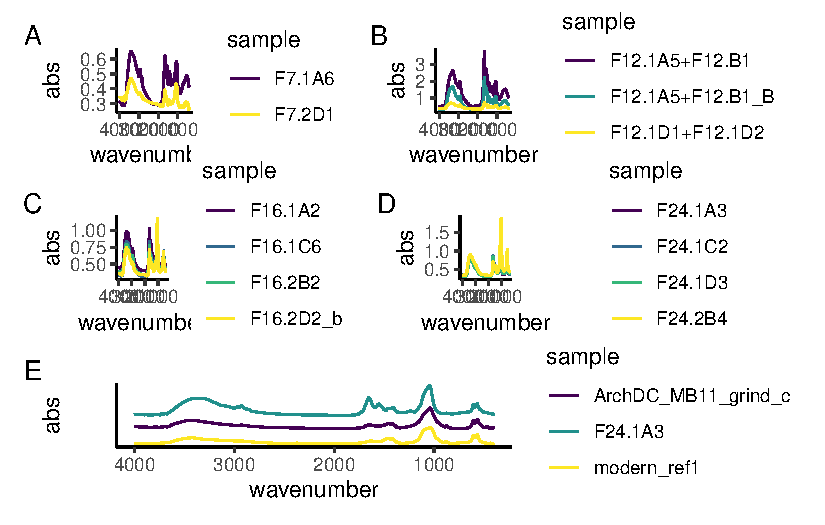
\includegraphics{figures/fig-experiment-spectra-1.pdf}

}

}

\subcaption{\label{fig-experiment-spectra-1}A}
\end{minipage}%
%
\begin{minipage}[t]{0.50\linewidth}

{\centering 

\raisebox{-\height}{

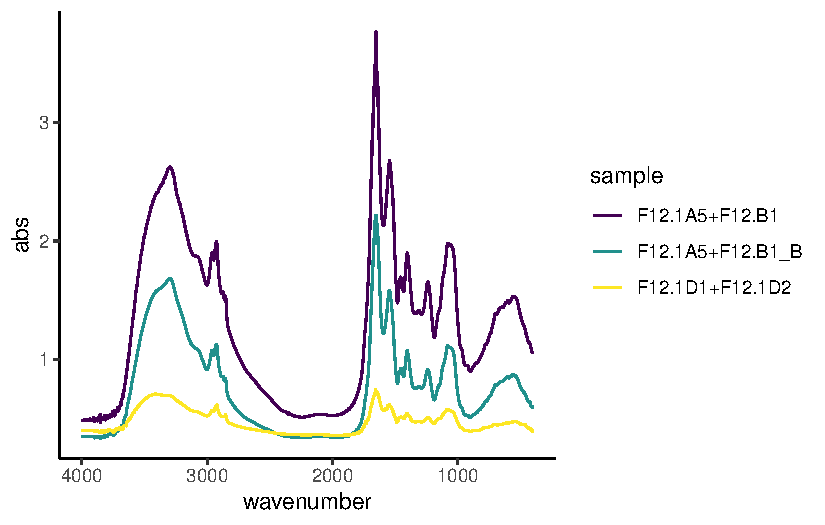
\includegraphics{figures/fig-experiment-spectra-2.pdf}

}

}

\subcaption{\label{fig-experiment-spectra-2}B}
\end{minipage}%
\newline
\begin{minipage}[t]{0.50\linewidth}

{\centering 

\raisebox{-\height}{

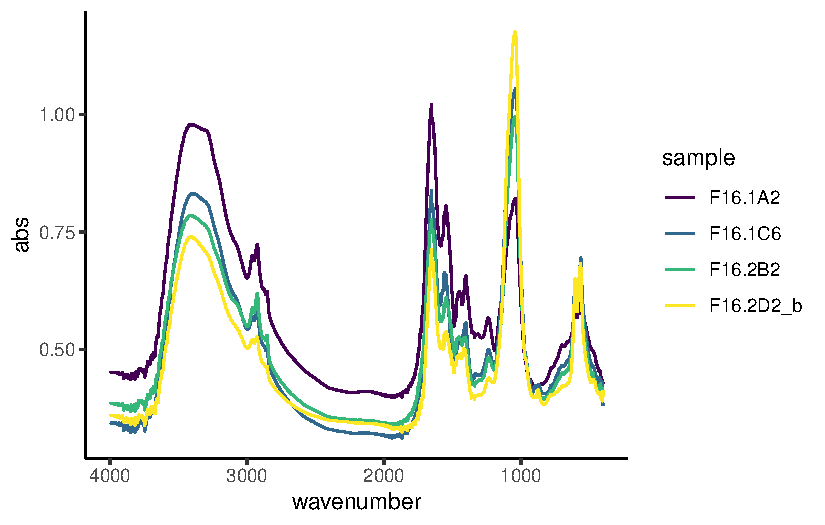
\includegraphics{figures/fig-experiment-spectra-3.pdf}

}

}

\subcaption{\label{fig-experiment-spectra-3}C}
\end{minipage}%
%
\begin{minipage}[t]{0.50\linewidth}

{\centering 

\raisebox{-\height}{

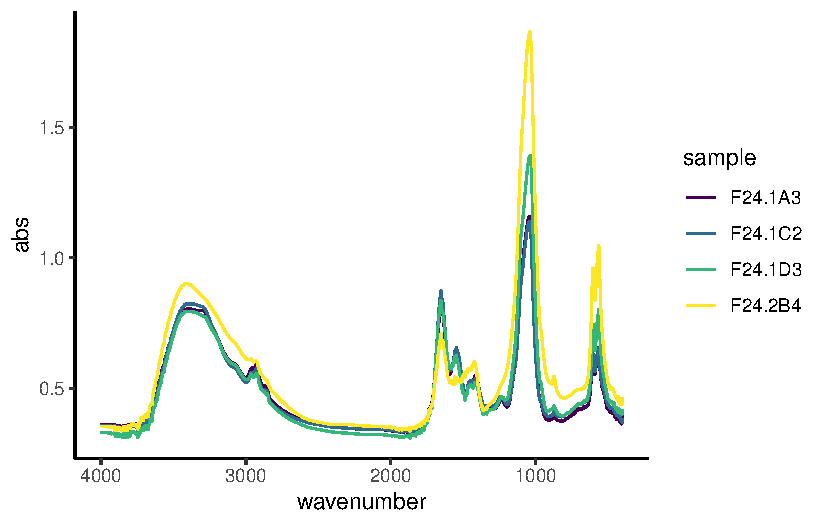
\includegraphics{figures/fig-experiment-spectra-4.pdf}

}

}

\subcaption{\label{fig-experiment-spectra-4}D}
\end{minipage}%

\caption{\label{fig-experiment-spectra}Select spectra from all
experiment sampling days.}

\end{figure}

Day 7 spectra have large O--H and amide A absorbance bands in stretching
mode around 3400 cm\(^{-1}\), as well as three marked
CH\textsubscript{3} and CH\(_2\) stretching vibrations at 2960, 2920,
and 2850 cm\(^{-1}\). There is a clear amide I peak at 1650 and a less
pronounced amide II peak at 1545 cm\(^{-1}\). In the `fingerprint'
region, C--O\(_3^{2-}\) at 1450 and 1400 absorbance bands corresponding
to the v\textsubscript{3} asummetric stretching vibrations,
P--O\textsubscript{4} absorbance band corresponding to the
v\textsubscript{3} asymmetric stretching vibrations at 1080 cm\(^{-1}\),
and minor phosphate absorption bands around 500 cm\(^{-1}\) in sample
F7.1A6, but absent in sample F7.2D1. The absorption bands at 1080
cm\(^{-1}\), and 1040-1047 cm\(^{-1}\) and minor bending absorption
bands of the phosphate doublet around 605 cm\(^{-1}\) and 560
cm\(^{-1}\) in sample F7.2D1, but absent in sample F7.1A6. The
absorption bands at 1080 cm\(^{-1}\) could be a C--N stretching mode
from aliphatic amines, but may also come from silicate contamination
(typical quartz doublet at 797, 780). The relative absorbance of O--H
and Amide I and II bands are higher than the phosphate bands,
representing a relatively higher content of lipids and proteins than
inorganic content. Large variation between spectra.

Day 12, amide I and II continue to be the dominant peaks, and a higher
ratio of both amide and O--H to PO\textsubscript{4} v\textsubscript{3}
absorbance bands. Three marked CH\textsubscript{3} and CH\(_2\)
stretching vibrations at 2960, 2920, and 2850 cm\(^{-1}\). Reduced
variation between two of the three spectra.

Day 16, the ratio of O--H and amides to PO\textsubscript{4} has shifted,
with the main peak shifting to the PO\textsubscript{4}
v\textsubscript{3} absorbance band at 1040 (except in sample F16.1A2). A
well-defined PO\textsubscript{4} doublet at 600 and 560 is present.
Small CO\(_3^{2-}\) asymmetric stretching at 1450 cm\(^{-1}\) and 1415
cm\(^{-1}\), and stretching vibrations at 875-870 cm\(^{-1}\). Decreased
variability between the spectra, with most spectra exhibiting a higher
phosphate-to-protein/lipid ratio.

Day 24, large O--H and amide A absorbance bands in stretching mode
around 3400 cm\(^{-1}\), as well as three minor CH\textsubscript{3} and
CH\(_2\) stretching vibrations at 2960, 2920, and 2850 cm\(^{-1}\). Main
peak of spectra is PO\textsubscript{4} v\textsubscript{3} at 1040
cm\(^{-1}\), well-defined PO\textsubscript{4} doublet at 600-550
cm\(^{-1}\). Amide I band, with small amide II and III bands. Carbonate
peaks also present. Very little variation between all of the spectra.

The main difference in the samples across the experiment, with
increasing age, is an increase in the main PO\textsubscript{4}
v\textsubscript{3} peak at around 1040 cm\(^{-1}\), appearance of the
phosphate doublet around 600 and 560 cm\(^{-1}\) between day 12 and 16,
an increase in the carbonate peaks at 1458-1450 cm\(^{-1}\) and
1415-1420 cm\(^{-1}\), an increase in the ratio of the Amide I/II to
peaks at around 1650 and 1540 cm\(^{-1}\), and a reduction of the
C--H\textsubscript{2} and C--H\textsubscript{3} stretching vibrations at
2960, 2920, and 2850 cm\(^{-1}\).

High lipid and protein content consistent with the presence of
extracellular polysaccharides and bacteria within a matrix. Microbial
DNA and RNA may be visible from peaks around 1200--800 cm\(^{-1}\) on
days 7 and 12, which are later obscured by the increasing phosphate peak
at 1040 cm\(^{-1}\) (\textbf{jainIsolationCharacterization2013?}). The
presence of water indicated by the O--H stretch is also consistent with
a biofilm, which is around 90\% water
(\textbf{bergerOralBiofilms2018?}). As the samples mature, the ratio of
proteins and lipids to phosphates shift from predominance of organic
content to inorganic content in the form of carbonated hydroxyapatite.

Early spectra, days 7 and 12, are also similar to collagen spectra, with
the OH absorbance band at around 3400 cm\(^{-1}\), amide I, II, and III
peaks at 1659, 1552, and 1240 cm\(^{-1}\), respectively
(\textbf{rohanizadehUltrastructuralStudy2005?};
\textbf{martinezcortizasLinkingStructural2020?}).

The archaeological and modern reference spectra are largely
indistinguishable and consist of an O--H absorbance band (3400
cm\(^{-1}\)), CH\textsubscript{3} bands (3000--2900 cm\(^{-1}\)),
carbonate (1420, 1458-1450, 875-870 cm\(^{-1}\)), amide I band (1650
cm\(^{-1}\)), and phosphates (1040, 604, 566 cm\(^{-1}\)).

The biofilm samples from the end of the experiment are similar to both
reference samples. The main difference is a lower organic component in
reference samples seen as a reduced amide I peak at around 1637 compared
to the carbonate peak at around 1420, and an absence of amide II and
III. Also a reduction in CH\textsubscript{3} bands at 3000-2900
cm\(^{-1}\).

\hypertarget{grinding-curves}{%
\subsubsection{Grinding curves}\label{grinding-curves}}

\begin{figure}

{\centering 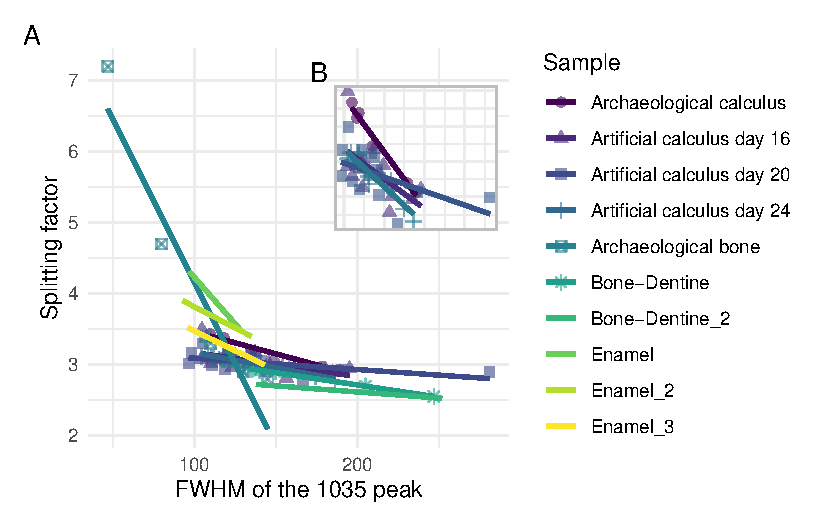
\includegraphics{figures/fig-grind-curve-inset-1.pdf}

}

\caption{\label{fig-grind-curve-inset}(A) Grinding curves of multiple
materials; and (B) calculus-only materials, including biofilm samples
from three days, and an archaeological calclulus sample.}

\end{figure}

Samples were compared to the results of
(\textbf{asscherAtomicDisorder2011?}) and
(\textbf{asscherVariationsAtomic2011?}), and the slopes of the trend
lines for our model calculus are similar to those of fresh bone and
dentin. No appreciable differences between days 16, 20, and 24. The
archaeological dental calculus does show a slightly increased slope
compared to model calculus from the three sampling days used in the
grind curve.

\hypertarget{discussion}{%
\section{Discussion}\label{discussion}}

\hypertarget{discussion-1}{%
\section{Discussion}\label{discussion-1}}

In this study we present a {[}long-term{]} oral biofilm model with
mineralisation to produce model dental calculus. The aim of the model is
to address a variety of research questions related to dental calculus,
both in the present and in the past. We also assess the viability of our
model as a proxy for dental calculus.

used metagenomic classification and FTIR to in bacterial and mineral
content. The performance of our model as a proxy for dental calculus was
evaluated using metagenomic screening for bacterial composition, and
FTIR for mineral structure.

While our model is not an anaerobic system, the anaerobes seem to have
outcompeted aerobes and facultative anaerobes over the course of the
experiment. This may be a result of biofilm microenvironments, where
species can produce favourable environments within biofilms.

Experimental samples are indicative of biofilm growth and maturation,
including mineralisation, represented by a reduction in proteins and
lipids (1460, 1420, 870) and the increasing intensity of peaks related
to carbonated hydroxyapatite (1040, 600-550 cm\(^{-1}\)) over the course
of the experiment.

The presence of collagen in dental calculus (and saliva) is still not
clear. It may be a result of external contamination
(\textbf{mackiePreservationMetaproteome2017?}) or end-products of
collagen degradation (e.g.~carboxyterminal telopeptide of type I
collagen, ICTP) which may or may not be related to periodontitis
(\textbf{gursoySalivaryCollagen2013?}). It is more likely that the
proline-rich proteins (secondary amine) present in the samples are
attributed to the biofilm matrix.

The artificial samples from day 24 resemble both the modern reference
samples and the archaeological sample in mineral composition and
crystallinity. The steeper slope of the archaeological sample may
suggest larger crystals, which is to be expected, as the inorganic
crystals expand into the space left by degrading organic matter over
time (\textbf{weinerBiologicalMaterials2010?}). More samples are needed
to see if this is consistent in archaeological samples. Overall, the
spectra of the artificial calculus show an increase in the inorganic
component and a decrease in the organic component over time. The
grinding curves for days 16, 20, and 24 were very similar, suggesting
that the CPMU solution (introduced on day 16) may not have much of an
effect.

Research relating to \(alpha\)-amylase activity and its effect on the
oral biome (whether dietary or otherwise) requires addition of amylase
to the microcosm, as it is not present in the naturally in the system
(as shown in ). The reason for the absence of \(alpha\)-amylase is not
clear\ldots{} There is of course no renewable source for
\(alpha\)-amylase once the inoculations have been completed;
furthermore, there does not seem to be any retention of
\(alpha\)-amylase by amylase-binding streptococci (ABS). ABS are present
in the system, but do not seem to be binding amylase. At this point we
are unable to explain why.

Single donor may have affected diversity of model. Donated saliva had a
lower mean alpha-diversity than other saliva samples.

This method can be used for a wide range of methods-testing (e.g.~DNA,
proteomics, etc.) as well as training for various sampling methods, and
contamination protocol testing. The model also has dietary applications,
which can be seen elsewhere .




\end{document}
